\chapter{Desenvolvimento da Ferramenta de Feedback Formativo - FeedFor}

\section{Visão Geral do Projeto}

O Projeto FeedFor é uma API desenvolvida para funcionar como uma ferramenta para disciplinas ou organizações que desejam uma integração maior com seus alunos, fornecendo feedbacks formativos que indicam por que as respostas estão erradas e o que pode ser estudado para melhorar naquele conteúdo. O projeto não se compromete com a correção das questões, mas sim com a revisão das respostas, mostrando os motivos dos erros e as ações necessárias para melhorar nas próximas avaliações sobre aquele assunto.

A função principal dessa ferramenta é fornecer feedbacks formativos, inicialmente planejados para servir apenas às disciplinas de Métodos de Desenvolvimento de Software e Requisitos de Software. No entanto, durante o desenvolvimento, o escopo foi ampliado, tornando a ferramenta genérica o suficiente para atender qualquer disciplina que deseje utilizá-la.

Dentro da ferramenta, é possível criar matérias, relacionar professores e alunos, e fornecer o contexto da disciplina para o assistente (OpenAI API). Também é possível usar qualquer modelo e configurações específicas desejadas no Chat, permitindo feedbacks mais individualizados.

O projeto FeedFor suporta diferentes tipos de questões, incluindo:

\begin{itemize}
    \item \textbf{Questões de Múltipla Escolha:} Onde os alunos selecionam uma única resposta correta entre várias opções.
    \item \textbf{Questões de Múltiplas Respostas Corretas:} Onde os alunos podem selecionar várias respostas corretas entre várias opções.
    \item \textbf{Questões Abertas:} Onde os alunos fornecem respostas discursivas, que são analisadas para gerar feedback formativo detalhado.
\end{itemize}

Com o escopo ampliado, outras funcionalidades secundárias foram adicionadas, incluindo:

\begin{itemize}
    \item \textbf{Autenticação:} A necessidade de autenticar os usuários para utilizar os serviços do FeedFor.
    \item \textbf{Reenvio de Feedback:} A possibilidade de reenviar feedbacks formativos recebidos ou enviá-los para outra pessoa.
    \item \textbf{Relatórios de Desempenho:} Um recurso gerencial que permite aos professores receber relatórios sobre o desempenho da turma e estatísticas sobre as questões criadas.
\end{itemize}

\section{Metodologia de Desenvolvimento}

Para o desenvolvimento da ferramenta FeedFor, utilizou-se a metodologia Kanban, uma abordagem ágil que se mostrou eficaz para o gerenciamento do projeto. A escolha do Kanban visou garantir uma visão clara das atividades em andamento e permitir uma gestão eficiente das tarefas e prazos. A plataforma Jira foi empregada como ferramenta de apoio para a implementação do Kanban. No Jira, as atividades foram organizadas em quadros Kanban, facilitando a visualização do fluxo de trabalho e o controle do progresso das tarefas.

\section{Riscos e Impactos}

Durante o desenvolvimento do projeto FeedFor, diversos riscos foram considerados, alguns não previstos aconteceram e impactaram o andamento do trabalho. Entre os principais acontecimentos enfrentados, destacam-se:

\begin{itemize}
    \item A saída inesperada de um membro da equipe teve um impacto significativo na carga de trabalho e na divisão de tarefas. A quantidade de trabalho planejada para duas pessoas precisou ser redistribuída, o que resultou em uma reavaliação dos prazos e no aumento da carga de trabalho para o membro restante.
    \item A greve que afetou a Universidade de Brasília durante todo o semestre de 2024.1 causou interrupções significativas nas atividades acadêmicas e afetou a continuidade do projeto. A greve resultou em atrasos e na necessidade de ajustar o cronograma original.
    \item Um acidente sofrido pelo orientador resultou em uma licença médica durante o período da greve e algumas semanas após.
\end{itemize}

Os impactos desses acontecimentos incluíram a necessidade de reorganizar as tarefas e ajustar os prazos de entrega, além de enfrentar desafios adicionais na gestão do projeto. A falta de orientação e a alteração na divisão do trabalho contribuíram para a complexidade do gerenciamento das atividades, exigindo um esforço adicional para garantir a conclusão bem-sucedida da ferramenta FeedFor.

\section{Tecnologias Utilizadas}

Durante o desenvolvimento do projeto FeedFor, diversas tecnologias foram empregadas para atender às necessidades específicas e melhorar a eficiência do sistema. Inicialmente, havia a intenção de utilizar o framework FastAPI, devido à sua alta performance e simplicidade. No entanto, ao longo do desenvolvimento, optou-se pelo framework Django, por oferecer configurações prontas que facilitaram o gerenciamento do projeto. Entre as vantagens do Django, destacam-se:

\begin{itemize}
    \item \textbf{Gerenciamento de Usuários:} Django vem com um sistema de autenticação e gerenciamento de usuários robusto e seguro, o que simplificou a implementação dessas funcionalidades.
    \item \textbf{Configurações Prontas:} O Django oferece uma estrutura pré-configurada que agiliza o desenvolvimento de aplicações web, incluindo roteamento, middleware e templates.
    \item \textbf{Biblioteca ORM:} A biblioteca de ORM (Object-Relational Mapping) do Django é robusta e flexível, facilitando a modelagem e o gerenciamento do banco de dados.
\end{itemize}

Além do Django, a ferramenta OpenAI API foi utilizada para gerar os feedbacks formativos. Foi integrada ao sistema para processar as respostas dos questionários e fornecer feedbacks personalizados aos alunos.

Para lidar com múltiplas tarefas e evitar o bloqueio da API devido ao grande número de requisições à API do GPT, foram utilizadas as seguintes tecnologias:

\begin{itemize}
    \item \textbf{Celery:} Uma biblioteca de gerenciamento de tarefas distribuídas que permitiu a execução assíncrona de tarefas, como o processamento das respostas e o envio de feedbacks.
    \item \textbf{Redis:} Um banco de dados em memória que foi usado como broker para o Celery, armazenando e gerenciando as filas de tarefas.
\end{itemize}

Além dessas tecnologias principais, outras bibliotecas específicas foram utilizadas para funcionalidades adicionais:

\begin{itemize}
    \item \textbf{Pandas:} Utilizada para a criação de relatórios detalhados sobre o desempenho da turma, facilitando a análise por parte dos professores.
    \item \textbf{WeasyPrint:} Uma biblioteca que converte HTML e CSS em PDFs, usada para gerar os relatórios de feedback que são enviados aos alunos por e-mail.
\end{itemize}

Para facilitar o desenvolvimento, implantação e gerenciamento do projeto, todo o sistema foi conteinerizado utilizando Docker e Docker Compose. Esses containers permitem uma configuração consistente e um ambiente isolado para a execução e lançamento (deploy) do projeto, simplificando a gestão e a escalabilidade do sistema. 

A combinação dessas tecnologias permitiu a criação de uma ferramenta eficiente e eficaz para a geração de feedbacks formativos, garantindo um sistema robusto e escalável.


\section{Principais Endpoints}

Neste projeto, foram desenvolvidos seis endpoints principais, cada um com uma função específica para garantir o funcionamento adequado da ferramenta FeedFor. A seguir, detalhamos cada um desses endpoints:

\begin{itemize}
    \item \textbf{/admin/:} O endpoint padrão do Django Admin, que já vem configurado no projeto Django. Este endpoint fornece acesso à página de administração, permitindo o gerenciamento do banco de dados e a administração do sistema.

    \item \textbf{/api/token/:} Endpoint para recuperação do token de acesso. O usuário deve fornecer suas credenciais (usuário e senha) para obter um token de acesso, que é necessário para autenticar e acessar os serviços do projeto.

    \item \textbf{/api/token/refresh/:} Endpoint para atualização do token de acesso. Quando o token de acesso expira ou está próximo de expirar, este endpoint pode ser utilizado para renovar o token, garantindo que o usuário mantenha o acesso aos serviços.

    \item \textbf{/api/feedback/:} O principal endpoint deste projeto. Este endpoint recebe os dados de um questionário preenchido por um aluno, processa esses dados, gera o feedback formativo e envia um e-mail com o feedback para o aluno correspondente.

    \item \textbf{/api/feedback/resend/:} Endpoint para reenvio de feedback formativo. Este endpoint permite que um feedback formativo previamente gerado seja reenviado, mediante a especificação do questionário e das pessoas que devem receber o feedback.

    \item \textbf{/api/reports/:} Endpoint para envio de relatórios sobre o desempenho da turma de um professor. Com base em um questionário específico, este endpoint gera e envia um relatório detalhado, incluindo notas dos alunos, porcentagem de acertos por questão e outras estatísticas relevantes.
\end{itemize}

Além desses endpoints principais, foi implementado um endpoint adicional para documentação técnica:

\begin{itemize}
    \item \textbf{/swagger/:} Endpoint que fornece uma documentação técnica detalhada de todos os endpoints disponíveis no projeto. Através deste endpoint, é possível visualizar os parâmetros esperados e os possíveis responses para cada endpoint, facilitando a compreensão e integração com a API.
\end{itemize}

Cada um desses endpoints desempenha um papel crucial no fluxo de funcionamento da ferramenta FeedFor, garantindo desde a administração do sistema até a geração e envio de feedbacks e relatórios detalhados. A documentação técnica acessível pelo endpoint /swagger/ auxilia na integração e uso da API por terceiros.

\section{Banco de Dados e Modelagem}

Durante o processo de desenvolvimento do projeto FeedFor, o banco de dados passou por três fases distintas, refletindo a evolução e a ampliação do escopo da ferramenta.

\subsection{Primeira Fase}

Na primeira fase do projeto, o banco de dados era limitado a três tabelas: Estudante, Questionário e Item. Nesta fase, o projeto estava direcionado às disciplinas de Métodos de Desenvolvimento de Software e Requisitos de Software. Devido ao contexto restrito de usabilidade, o banco de dados foi desenvolvido de forma muito situacional.

\begin{figure}[H]
    \centering
    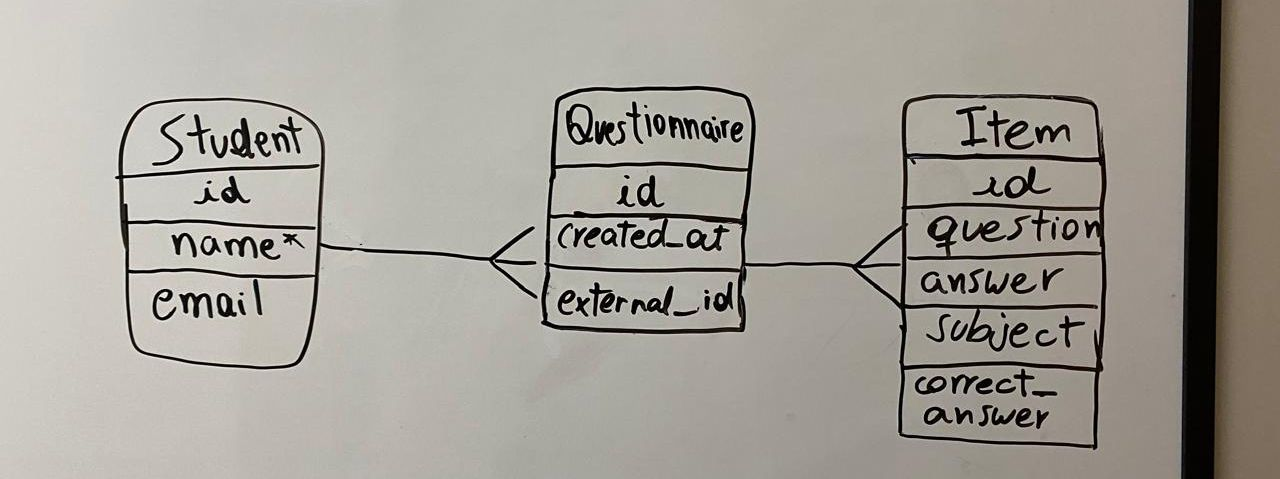
\includegraphics[width=0.8\textwidth]{figuras/bd-phase1.jpeg}
    \caption{Modelo de Banco de Dados - Primeira Fase}
    \label{fig:first_phase}
\end{figure}

O principal problema da primeira fase era a não reutilização dos feedbacks para cada questão. Quando uma resposta errada era recebida, uma nova requisição era feita à API da OpenAI para gerar o feedback, o que resultava em múltiplas requisições idênticas para a mesma questão em uma sala com muitos alunos.

\subsection{Segunda Fase}

Na segunda fase, foi criada uma tabela adicional de Respostas para armazenar os feedbacks gerados para respostas incorretas, evitando requisições redundantes à API da OpenAI. Além disso, alguns relacionamentos foram ajustados para suportar essa nova funcionalidade.

\begin{figure}[H]
    \centering
    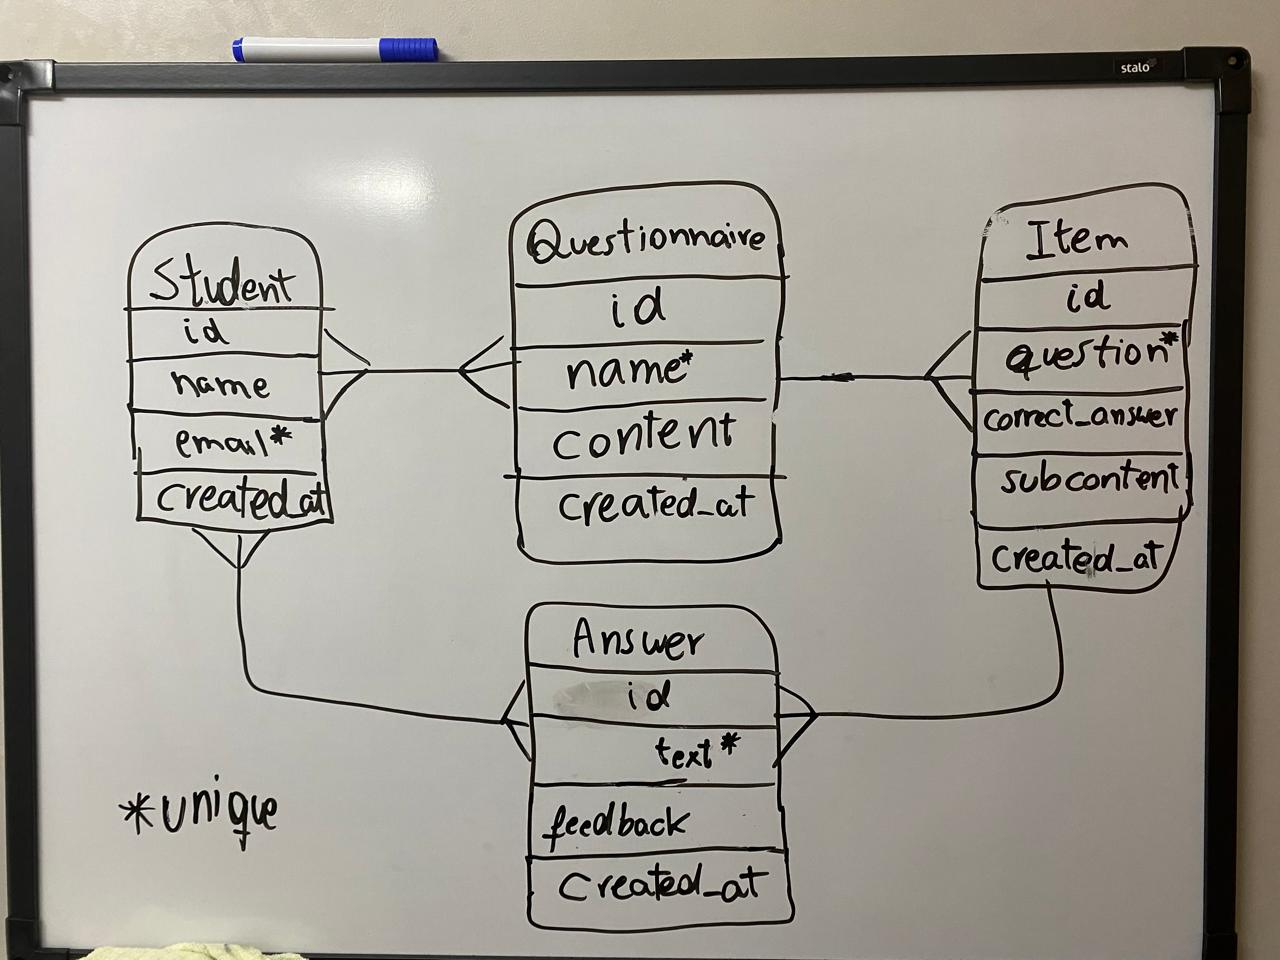
\includegraphics[width=0.8\textwidth]{figuras/bd-phase2.jpeg}
    \caption{Modelo de Banco de Dados - Segunda Fase}
    \label{fig:second_phase}
\end{figure}

Nesta versão, o banco de dados já atendia bem às disciplinas inicialmente desejadas. No entanto, devido ao tempo maior de desenvolvimento e ao entusiasmo do desenvolvedor com o projeto, decidiu-se ampliar o escopo para torná-lo mais genérico e aceitar múltiplas disciplinas trabalhando em conjunto.

\subsection{Terceira Fase}

Na terceira fase, foram feitos ajustes nos relacionamentos e adicionadas novas tabelas de Resultados, Matérias, Professores e Configurações do Chat. Isso permitiu um gerenciamento mais robusto e a divisão de questionários por matérias e professores, além de permitir que cada turma tivesse um chat personalizado com configurações específicas.

\begin{figure}[H]
    \centering
    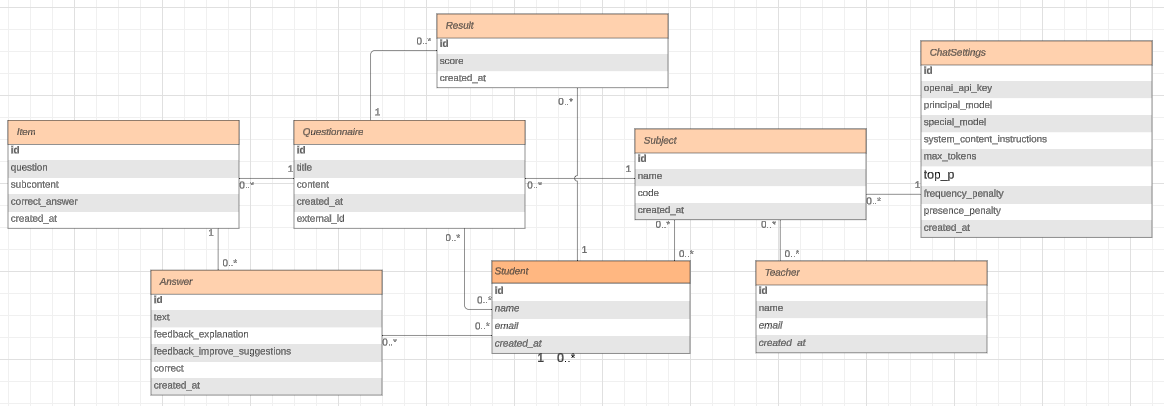
\includegraphics[width=1\textwidth]{figuras/bd-phase3.png}
    \caption{Modelo de Banco de Dados - Terceira Fase}
    \label{fig:third_phase}
\end{figure}

Para acessar o modelo dessa terceira fase basta acessar o link: \href{https://lucid.app/lucidchart/c1e592ab-3b4a-4bba-9849-cc3237f4fa76/edit?viewport_loc=-2447%2C-1073%2C2164%2C956%2C0_0&invitationId=inv_fbaaf515-3973-4d6a-9359-eb0dc4a26eee}{Modelo de Banco de Dados - Terceira Fase}.

\subsection{Explicação das Tabelas}

\begin{itemize}
    \item \textbf{Estudante (Student):} Armazena informações dos estudantes, sendo crucial o email para o envio dos feedbacks formativos.
    \item \textbf{Professor (Teacher):} Armazena informações dos professores, incluindo o email para receber relatórios de questionários e visualizar os feedbacks recebidos pelos alunos.
    \item \textbf{Matéria (Subject):} Armazena informações das matérias, ajudando a separar os contextos dos questionários e relacionando-se com as configurações do chat para determinar como os feedbacks serão gerados para aquela matéria.
    \item \textbf{Questionário (Questionnaire):} Armazena informações sobre os questionários realizados, incluindo o ID externo usado para regenerar feedbacks específicos.
    \item \textbf{Item (Item):} Armazena informações sobre as perguntas das questões, incluindo o conteúdo e a resposta correta, essenciais para contextualizar o feedback gerado pela API da OpenAI.
    \item \textbf{Resposta (Answer):} Armazena informações sobre as respostas dos alunos, indicando se estão corretas ou não e, se incorretas, os feedbacks gerados, permitindo a reutilização futura do feedback.
    \item \textbf{Resultado (Result):} Armazena a pontuação obtida por um aluno em um questionário.
    \item \textbf{Configurações do Chat (ChatSettings):} Armazena configurações do modelo requisitado na API da OpenAI, como a versão do modelo, temperatura, token de acesso à API e outras configurações técnicas.
\end{itemize}

\section{Arquitetura do Sistema}

Inicialmente, o projeto FeedFor foi planejado para utilizar a Arquitetura Limpa no Django. A Arquitetura Limpa, também conhecida como Clean Architecture, é um estilo de arquitetura de software que promove a separação de preocupações e a independência das camadas do sistema. Em uma Arquitetura Limpa, a lógica de negócios é isolada das preocupações com o acesso a dados e interfaces externas, permitindo maior flexibilidade e facilidade na manutenção e teste do sistema. Esse tipo de arquitetura busca garantir que o núcleo da aplicação permaneça independente de frameworks e bibliotecas específicas, o que facilita a evolução e adaptação da aplicação ao longo do tempo \cite{tabnews2023}.

No entanto, ao longo do desenvolvimento do projeto, e após a saída de um dos desenvolvedores, optou-se por seguir uma abordagem de Arquitetura em Camadas mais simples. Esta arquitetura é uma abordagem mais tradicional, que organiza o sistema em camadas distintas, cada uma com responsabilidades específicas:

\begin{itemize}
    \item \textbf{Camada de Acesso a Dados:} Responsável por interagir com o banco de dados. Essa camada é encarregada de realizar operações de leitura e escrita nos dados, garantindo que as regras de negócio não sejam diretamente afetadas pelas operações de armazenamento.
    \item \textbf{Camada de Processamento Interno:} Encarregada de implementar a lógica de negócios da aplicação. Esta camada processa as informações recebidas e realiza as operações necessárias para gerar o feedback formativo, isolando a lógica de negócio da camada de acesso a dados e das comunicações externas.
    \item \textbf{Camada de Comunicação Externa:} Responsável por interagir com sistemas externos, como APIs externas e serviços de email. Esta camada gerencia as requisições a serviços externos, como a API da OpenAI para geração de feedbacks e o envio de emails para os alunos.
\end{itemize}

A Arquitetura em Camadas foi escolhida devido à sua simplicidade e adequação ao contexto do projeto após a mudança na equipe. Embora não ofereça a mesma flexibilidade e independência da Arquitetura Limpa, ela permite uma organização clara das responsabilidades e facilita a manutenção e evolução da aplicação com a equipe reduzida.

\section{Custos do Projeto}

O desenvolvimento e a operação do projeto FeedFor envolvem alguns custos principais, que estão relacionados principalmente ao uso da OpenAI API e à hospedagem do projeto. A seguir, apresentamos uma análise detalhada desses custos.

\subsection{Custo da OpenAI API}

O principal custo associado ao FeedFor é o uso da OpenAI API, que não é mais gratuita para novos usuários. Durante a fase de testes do projeto, foi gasto um total de 5 dólares, o valor mínimo para adquirir créditos na plataforma. Desses 5 dólares, foram utilizados efetivamente 0.24 dólares para 225 requisições.

O custo da OpenAI API é baseado na quantidade de tokens processados e qual modelo é utilizado. Tokens são sequências de caracteres que podem representar palavras, partes de palavras ou até mesmo caracteres individuais, dependendo do contexto. O projeto, em média, utiliza cerca de 500 tokens por requisição (entrada e saída), o que resulta em um custo relativamente baixo.

Vale destacar que durante os testes, mais da metade dos gastos foram com o modelo mais recente da OpenAI, que possui um custo mais elevado em comparação ao modelo GPT-3.5-turbo. O GPT-3.5-turbo demonstrou ser suficiente para as necessidades do projeto e tem um custo mais acessível, o que indica que os gastos reais podem ser ainda menores no uso contínuo.

Inicialmente, o custo pode ser um pouco mais alto devido ao fato de que nenhuma questão terá um feedback pré-preenchido. Cada nova resposta errada gera uma nova requisição à API. No entanto, com o tempo, à medida que mais feedbacks forem gerados e armazenados, o número de novas requisições será reduzido, resultando em uma diminuição significativa dos custos operacionais.

\subsection{Custo de Hospedagem}

Além dos custos com a API, há também o custo de manter o projeto FeedFor hospedado em um serviço na nuvem. A Universidade de Brasília já possui servidores para serviços internos, mas, caso fosse necessário utilizar serviços externos, o Google Cloud Platform (GCP) foi utilizado para estimar os custos. Durante 4 semanas de hospedagem com um uso moderado dos serviços de VM e Storage, o gasto foi de 1.4 dólares. Como o GCP oferece um crédito gratuito de 300 dólares, o projeto teria um período considerável para testar a plataforma e avaliar a melhor opção para hospedagem.

\subsection{Resumo dos Custos}

- \textbf{OpenAI API:} Estimado em 0.24 dólares por 225 requisições, com um custo maior inicial que se reduzirá com o tempo.

- \textbf{Hospedagem em Nuvem:} Aproximadamente 1.4 dólares para 4 semanas de uso moderado no Google Cloud Platform, com a possibilidade de testes prolongados devido ao crédito gratuito.

Em resumo, os custos do projeto FeedFor são relativamente baixos, especialmente em comparação com os benefícios proporcionados pela ferramenta. A gestão eficiente das requisições à API e a escolha de opções de hospedagem adequadas contribuem para a sustentabilidade econômica do projeto.

\section{Uso da OpenAI API}

A OpenAI API é uma peça fundamental do projeto FeedFor, utilizada para gerar feedbacks formativos para as respostas dos alunos. A seguir, detalhamos como a API é empregada e os desafios enfrentados durante sua integração.

\subsection{Geração de Feedbacks}

A OpenAI API é acionada sempre que uma nova resposta incorreta é recebida e não está previamente armazenada no banco de dados. Dependendo do tipo de questão (múltipla escolha, aberta e múltiplas respostas corretas), o prompt enviado para a API varia para garantir a melhor contextualização possível. Essa abordagem foi desenvolvida após centenas de testes para otimizar a qualidade dos feedbacks gerados, inicialmente era planejado usar o mesmo prompt, mas com os testes foi identificado uma melhora ao descrever melhor cada contexto.

\subsubsection{Questões de Múltipla Escolha e Abertas}

Para questões de múltipla escolha ou abertas, o prompt enviado à OpenAI API inclui os seguintes campos:

- \textbf{Questão:} O texto da pergunta feita ao aluno.

- \textbf{Resposta do Aluno:} A resposta fornecida pelo aluno.

- \textbf{Gabarito:} A resposta correta para a questão.

- \textbf{Conteúdo do Questionário:} O conteúdo associado ao questionário no qual a questão está inserida.

- \textbf{Subconteúdo da Questão:} Detalhes adicionais relacionados à questão específica.

O prompt solicita que a API explique por que a resposta do aluno está incorreta, qual seria a resposta certa e sugira formas de estudo para melhorar o desempenho do aluno. A resposta é dividida em duas seções: \textit{Explicação} e \textit{Sugestões de Aperfeiçoamento}.

\subsubsection{Questões com Múltiplas Respostas Corretas}

Para questões que permitem múltiplas respostas corretas, o prompt inclui:

- \textbf{Questão:} O texto da pergunta.

- \textbf{Respostas do Aluno:} Lista das respostas do aluno, separadas em \textit{Certas} e \textit{Erradas}.

- \textbf{Gabarito:} A lista das respostas corretas.

- \textbf{Conteúdo do Questionário:} O conteúdo associado ao questionário.

- \textbf{Subconteúdo da Questão:} Detalhes adicionais sobre a questão.

Este prompt solicita um feedback detalhado sobre as respostas fornecidas, dividido em \textit{Explicação} e \textit{Sugestões de Aperfeiçoamento}, considerando as respostas e o conteúdo associado à questão.

\subsection{Escolha de Modelos}

Durante o desenvolvimento, observou-se que o modelo GPT-3.5-turbo, embora eficiente para questões com múltiplas respostas corretas, foi superado pelo modelo mais recente da OpenAI em termos de qualidade de feedback. Portanto, o líder da disciplina pode escolher qual modelo utilizar para cada tipo de questão. A modelagem dos dados, como descrito na seção de Banco de Dados, inclui o campo \texttt{special\_model} na tabela \texttt{ChatSettings}, que permite selecionar um modelo diferente para questões com múltiplas respostas corretas, se desejado.

\subsection{Configurações e Desafios}

Alguns desafios foram enfrentados ao trabalhar com a OpenAI API:

- \textbf{Temperatura do Modelo:} A temperatura é um parâmetro que controla a aleatoriedade das respostas. Para evitar respostas imprecisas, a configuração da temperatura é ajustada para 0.0, garantindo respostas baseadas em fatos conhecidos e minimizando especulações.

- \textbf{Formatação de Respostas:} Para evitar problemas com caracteres especiais e formatação inadequada, são incluídas instruções específicas no prompt para assegurar que as respostas sejam claras e formatadas corretamente.

- \textbf{Controle de Tokens:} A quantidade de tokens na resposta pode variar. Para garantir que o feedback não seja cortado abruptamente, é enviado um limite de tokens definidos na tabela \texttt{ChatSettings} mais 50 (200 tokens definidos + 50 tokens adicionais por exemplo), ajustando automaticamente para evitar cortes indesejados.

Esses ajustes e configurações foram desenvolvidos para aprimorar a eficácia da API e garantir que os feedbacks gerados atendam às necessidades do projeto FeedFor.

\section{Definição do Template do Feedback Formativo}

O Feedback Formativo é um componente crucial para o aprendizado dos alunos, proporcionando informações detalhadas sobre suas respostas e orientações para melhorar seu desempenho. O desenvolvimento do template do feedback passou por várias fases, e a versão final foi definida com base em avaliações de profissionais da área da educação e especialistas em atendimento a pessoas com transtornos do neurodesenvolvimento.

\subsection{Exemplos de Feedback Formativo}

A seguir, são apresentadas duas imagens exemplificando o formato final do Feedback Formativo recebido pelos alunos:

\begin{figure}[H]
    \centering
    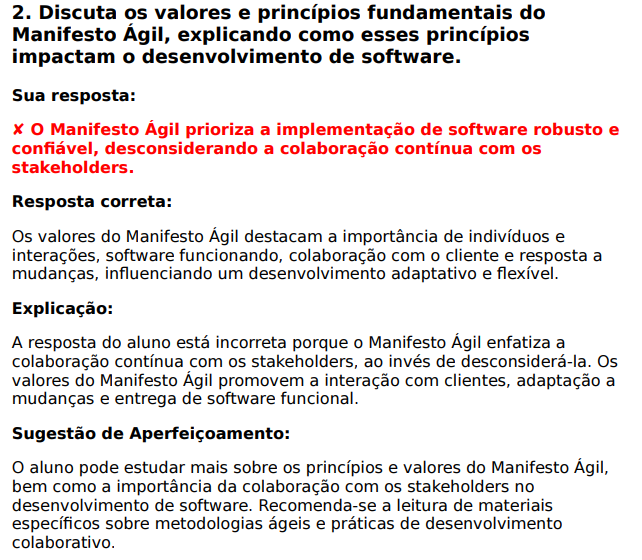
\includegraphics[width=1\textwidth]{figuras/feedback-example1.png}
    \caption{Exemplo de Feedback Formativo - Questão Errada}
    \label{fig:feedback_example1}
\end{figure}

\begin{figure}[H]
    \centering
    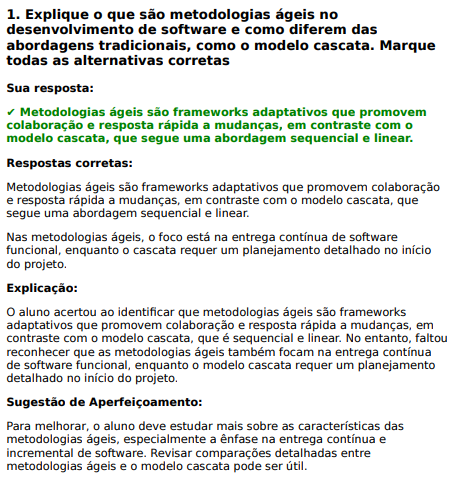
\includegraphics[width=1\textwidth]{figuras/feedback-example2.png}
    \caption{Exemplo de Feedback Formativo - Questão Correta}
    \label{fig:feedback_example2}
\end{figure}

\subsection{Design e Cores do Feedback}

Para garantir uma comunicação clara e intuitiva, foram selecionadas cores específicas para representar a correção das respostas:

- \textbf{Vermelho:} Utilizado para indicar respostas incorretas, destacando as áreas onde o aluno cometeu erros.

- \textbf{Verde:} Utilizado para indicar respostas corretas, reconhecendo o desempenho adequado do aluno.

Quando uma questão permite múltiplas respostas, as cores podem aparecer simultaneamente para distinguir entre respostas corretas e incorretas.

\subsection{Estrutura do Feedback}

A estrutura do feedback foi cuidadosamente elaborada para facilitar a compreensão e a leitura dos alunos. O template final foi definido da seguinte forma:

1. \textbf{Resposta Correta:} A(s) resposta(s) correta(s) é(são) exibida(s) primeiramente, para que o aluno saiba o que deveria ter sido a resposta correta.

2. \textbf{Explicação do Erro:} Após a apresentação da resposta correta, é fornecida uma explicação detalhada sobre por que a resposta do aluno estava incorreta. Essa seção busca esclarecer o erro e ajudar o aluno a entender o conceito de forma mais aprofundada.

3. \textbf{Sugestões de Aperfeiçoamento:} Em seguida, são apresentadas sugestões específicas sobre o que o aluno pode estudar ou melhorar para evitar erros semelhantes no futuro. Essas sugestões são separadas em textos curtos para facilitar a leitura e a compreensão.

O tamanho das respostas foi definido para ter um máximo de \textbf{200 tokens}. Esse limite foi escolhido com base em testes e avaliações de usabilidade, considerando que 200 tokens representam um tamanho adequado para a leitura e compreensão dos alunos, proporcionando um feedback claro e conciso sem sobrecarregar o estudante com informações excessivas, porém, se o professor desejar maiores feedbacks também é possível.

A separação dos textos em respostas corretas, explicações e sugestões visa incentivar a leitura e a assimilação de informações mais curtas e objetivas, especialmente para alunos que podem precisar de uma abordagem mais direta para absorver o conteúdo.

Este formato foi escolhido para maximizar a eficácia do feedback formativo, ajudando os alunos a identificar e corrigir suas falhas de forma clara e prática.

\section{Ideias Descartadas e Potenciais para Evolução}

Durante o desenvolvimento do projeto FeedFor, diversas ideias e recursos foram considerados e testados para aprimorar a funcionalidade da ferramenta. Algumas dessas ideias foram eventualmente descartadas devido a limitações técnicas ou falta de benefícios claros em relação à abordagem atual. No entanto, elas podem representar oportunidades valiosas para futuras versões do projeto.

\subsection{Utilização de Assistentes da OpenAI API}

Uma das ideias descartadas foi a utilização de assistentes da OpenAI API que, conforme a documentação da plataforma, permite o upload de documentos, como imagens ou PDFs, para usar como base para a interação com os alunos. A proposta era integrar esse recurso para fornecer feedbacks ainda mais personalizados, baseados em materiais específicos da disciplina fornecidos pelos professores.

Durante o desenvolvimento, foram encontradas várias dificuldades com essa abordagem:

- \textbf{Conexão Persistente:} O assistente da OpenAI API não mantinha as informações dos documentos carregados após uma perda de conexão. Isso significava que, se a conexão com o chat do assistente fosse perdida, as informações dos documentos não eram retidas, tornando a solução onerosa e difícil de gerenciar para a aplicação.
  
- \textbf{Armazenamento e Custo:} Manter a conectividade constante com o assistente para garantir que as informações dos documentos fossem preservadas seria custoso e complexo, o que não justificava os benefícios no contexto do projeto.

Embora esse recurso estivesse em fase beta durante o desenvolvimento, e tenha mostrado potencial para uma personalização ainda mais aprofundada dos feedbacks, os desafios encontrados levaram à decisão de optar por uma abordagem mais direta e confiável.

\subsection{Implementação e Configuração dos Assistentes}

Durante o desenvolvimento, a comunicação da aplicação com a OpenAI API foi completamente implementada, permitindo a criação, edição e exclusão de assistentes diretamente pela página de administração do FeedFor. Foi possível também realizar o upload de documentos para esses assistentes.

No entanto, essa funcionalidade foi removida do projeto final, pois não ofereceu vantagens significativas em relação ao uso do Chat normal, que já proporcionava o feedback necessário de forma eficiente e confiável.

\subsection{Potenciais para Futuras Versões}

Apesar das dificuldades enfrentadas com o recurso de assistentes, ele representa uma área promissora para futuras evoluções do projeto. Em versões posteriores, se melhorias forem implementadas na manutenção de estado e conectividade ou armazenamento de chats anteriores, o uso de assistentes com documentos personalizados pode adicionar um valor significativo ao FeedFor. A capacidade de fornecer feedbacks baseados em materiais específicos da matéria, como notas de aula e PDFs, poderia enriquecer ainda mais a experiência de aprendizado dos alunos.

O acompanhamento das atualizações e melhorias nas APIs e recursos da OpenAI, bem como a adaptação das soluções tecnológicas à medida que o projeto evolui, pode abrir novas possibilidades para incorporar essas ideias descartadas de maneira eficiente e benéfica.

